\documentclass[conference]{IEEEtran}
\usepackage{times}

% numbers option provides compact numerical references in the text. 
\usepackage[numbers]{natbib}
\usepackage{multicol}
\usepackage[bookmarks=true]{hyperref}
\usepackage{color}
\usepackage{amsmath}
\usepackage{amssymb}
\usepackage{booktabs}
\usepackage{mathtools}
\usepackage{graphicx}
\usepackage{graphicx}
\usepackage{caption}
\usepackage{subcaption}
% Variables used across report
\newcommand{\actionset}{\ensuremath{\mathcal{A}}}
\newcommand{\actionsetsize}{\ensuremath{|\mathcal{A}|}}
\newcommand{\actionvar}{\ensuremath{a}}
\newcommand{\actionsub}[1]{\ensuremath{a_{#1}}}
\newcommand{\actionsubsup}[2]{\ensuremath{a_{#1}^{#2}}}

\newcommand{\demoset}{\ensuremath{\mathcal{D}}}
\newcommand{\demovar}{\ensuremath{d}}
\newcommand{\demosub}[1]{\ensuremath{d_{#1}}}
\newcommand{\demosubsup}[2]{\ensuremath{d_{#1}^{#2}}}

\newcommand{\trajset}{\ensuremath{\mathcal{T}}}

\newcommand{\labelset}{\ensuremath{\mathcal{L}}}
\newcommand{\labelsetsize}{\ensuremath{|\mathcal{L}|}}
\newcommand{\labelvar}{\ensuremath{\ell}}
\newcommand{\labelsub}[1]{\ensuremath{l_{#1}}}
\newcommand{\nsub}[1]{\ensuremath{n_{#1}}}
\newcommand{\sapairsub}[1]{\ensuremath{(s_{#1}, a_{#1})}}

\newcommand{\stateset}{\ensuremath{\mathcal{S}}}
\newcommand{\statevar}{\ensuremath{s}}
\newcommand{\statesub}[1]{\ensuremath{s_{#1}}}
\newcommand{\statesubsup}[2]{\ensuremath{s_{#1}^{#2}}}
\newcommand{\nextstatevar}{\ensuremath{s'}}
\newcommand{\transitionfn}{\ensuremath{T}}
\newcommand{\rewardfn}[1]{\ensuremath{R}}
\newcommand{\goalset}{\ensuremath{\mathcal{G}}}

\newcommand{\policyset}{\ensuremath{{\Pi}}}
\newcommand{\policyvar}{\ensuremath{\pi}}
\newcommand{\policysub}[2]{\ensuremath{\pi_{#1}(#2)}}

\newcommand{\regcost}{\ensuremath{r}}
\newcommand{\indexvar}{\ensuremath{i}}

\newcommand{\landmarkset}{\ensuremath{\mathcal{K}}}

\newcommand{\marginvar}{\ensuremath{m}}
\newcommand{\approxq}{\ensuremath{\tilde{Q}}}
\newcommand{\weights}{\ensuremath{w}}
\newcommand{\weightszero}{\ensuremath{w_0}}
\newcommand{\weightst}{\ensuremath{w^\intercal}}
\newcommand{\featurefn}{\ensuremath{\phi}}
\newcommand{\features}[2]{\ensuremath{\phi({#1}, {#2})}}
\newcommand{\marginslackc}{\ensuremath{C}}
\newcommand{\marginslacksubsup}[2]{\ensuremath{\xi_{#1}^{#2}}}
\newcommand{\bellmanslackc}{\ensuremath{D}}
\newcommand{\bellmanslacksubsup}[2]{\ensuremath{\nu_{#1}^{#2}}}
\newcommand{\bellmanc}{\ensuremath{F}}


\pdfinfo{
   /Author (Homer Simpson)
   /Title  (Robots: Our new overlords)
   /CreationDate (D:20101201120000)
   /Subject (Robots)
   /Keywords (Robots;Overlords)
}

\DeclareMathOperator*{\argmin}{argmin}
\DeclareMathOperator*{\argmax}{argmax}

\newcommand{\et}[1]{\textcolor{blue}{Eric: #1}}
\newcommand{\dhm}[1]{\textcolor{red}{Dylan: #1}}
\newcommand{\sh}[1]{\textcolor{green}{Sandy: #1}}
\newcommand{\al}[1]{\textcolor{magenta}{Alex: #1}}

\begin{document}
% paper title
%\title{A Max-Margin Q-Learning Approach to Learning from Multiple Demonstrations}
%\title{Max-Margin Q-Learning:\\ {\huge An Approach to Learning from Multiple Demonstrations}}
\title{Max-Margin Q-Learning with Application to Manipulation of Deformable Objects}
% Learning to Use Expert Demonstrations

% You will get a Paper-ID when submitting a pdf file to the conference system
\author{Dylan Hadfield-Menell, Alex Lee, Sandy Huang, Eric Tzeng, and Pieter Abbeel}

%\author{\authorblockN{Michael Shell}
%\authorblockA{School of Electrical and\\Computer Engineering\\
%Georgia Institute of Technology\\
%Atlanta, Georgia 30332--0250\\
%Email: mshell@ece.gatech.edu}
%\and
%\authorblockN{Homer Simpson}
%\authorblockA{Twentieth Century Fox\\
%Springfield, USA\\
%Email: homer@thesimpsons.com}
%\and
%\authorblockN{James Kirk\\ and Montgomery Scott}
%\authorblockA{Starfleet Academy\\
%San Francisco, California 96678-2391\\
%Telephone: (800) 555--1212\\
%Fax: (888) 555--1212}}


% avoiding spaces at the end of the author lines is not a problem with
% conference papers because we don't use \thanks or \IEEEmembership


% for over three affiliations, or if they all won't fit within the width
% of the page, use this alternative format:
% 
%\author{\authorblockN{Michael Shell\authorrefmark{1},
%Homer Simpson\authorrefmark{2},
%James Kirk\authorrefmark{3}, 
%Montgomery Scott\authorrefmark{3} and
%Eldon Tyrell\authorrefmark{4}}
%\authorblockA{\authorrefmark{1}School of Electrical and Computer Engineering\\
%Georgia Institute of Technology,
%Atlanta, Georgia 30332--0250\\ Email: mshell@ece.gatech.edu}
%\authorblockA{\authorrefmark{2}Twentieth Century Fox, Springfield, USA\\
%Email: homer@thesimpsons.com}
%\authorblockA{\authorrefmark{3}Starfleet Academy, San Francisco, California 96678-2391\\
%Telephone: (800) 555--1212, Fax: (888) 555--1212}
%\authorblockA{\authorrefmark{4}Tyrell Inc., 123 Replicant Street, Los Angeles, California 90210--4321}}


\maketitle

%% \begin{abstract}
%% We consider the problem of learning from demonstrations
%% to manipulate deformable objects. Recent
%% work~\cite{Schulmanetal_IROS2013, Schulmanetal_ISRR2013} has shown
%% promising results in enabling robotic manipulation of deformable
%% objects through learning from demonstrations.  Their approach is able
%% to generalize from a single demonstration to new test situations,
%% and suggests a nearest
%% neighbor approach to decide which demonstration to generalize from for
%% a given test situation.  Such a nearest neighbor approach, however,
%% ignores important aspects of the problem:  brittleness (versus
%% robustness) of demonstrations when generalized through this process,
%% and the extent to which a demonstration makes progress towards the goal.

%% In this paper, we present a max-margin q-learning-based solution
%% to the demonstration selection problem that
%% can account for the variability in robustness of demonstrations and the
%% sequential nature of our tasks.   We also present experimental
%% validation of our approach.  We developed a knot-tying benchmark for
%% evaluating the effectiveness of
%% our proposed approach.   The
%% nearest neighbor approach described in \citet{Schulmanetal_ISRR2013} achieves a
%% 68.8\% success rate. Our approach achieves a success rate of 95.2\%.
%% \end{abstract}

Automated manipulation of deformable objects tends to be challenging
due to high-dimensional, continuous state-action spaces and due to the
complicated dynamics of deformable objects. Direct planning or optimal
control techniques are often intractable for this setting.

Despite these challenges, recent work~\cite{Schulmanetal_IROS2013,
  Schulmanetal_ISRR2013} has leveraged expert demonstrations to make
progress on robotic manipulation of deformable objects. This work uses
non-rigid registration between a demonstration scene and a test scene
to find a geometric mapping between the demonstration and test scene.
This mapping is used to perform \emph{trajectory transfer} for the
demonstrated gripper trajectory. This approach has been validated in
simulated and real-world environments for knot-tying, suturing, and
folding tasks.

In particular, this method of trajectory transfer uses a thin-plate
spline (TPS) to find a mapping between these two scenes. A TPS
minimizes the curvature of the mapping function and will (hopefully)
find a mapping, or warping, that is close to rigid. This is motivated
by the observation that for many tasks, success in a task is preserved
over Euclidean transformation. Furthermore, the associated
optimization problem can be solved efficiently~\cite{Wahba_TPS1990}.

Full demonstrations of complex tasks with multiple steps will be hard
to collect and transfer successfully. As such, we assume that
demonstrations often correspond to steps in the task, rather than the
entire task itself. Figure~\ref{fig:knot_steps} shows an example of
the steps involved in tying an overhand knot. Furthermore, a single demonstration
for a step in the task cannot be expected to cover all possible
scenarios that arise during execution.  The natural solution to this
is to use a library of demonstrations with multiple demonstrations for
each step.

Realizing these benefits requires a robust technique to select a good
trajectory to transfer.  Certain trajectories will generalize better
than others, and particular sequences of demonstrations may perform
tasks more efficiently than others.

The original paper on the approach of trajectory transfer
prescribes choosing the trajectory segment from the demonstrations
library with the lowest warping cost onto the current
scene~\cite{Schulmanetal_ISRR2013}.  This approach does not account
for the inherent generalizability of a particular demonstration. For
brittle demonstrations (e.g. grabbing near the edge of a rope), a
small change in the rope can have low registration cost, but the
transferred trajectory will fail.  As a result, such an approach may
fail to accomplish tasks that would be possible with a different
sequence of trajectories.

\begin{figure}[t]
  \centering
    \noindent
    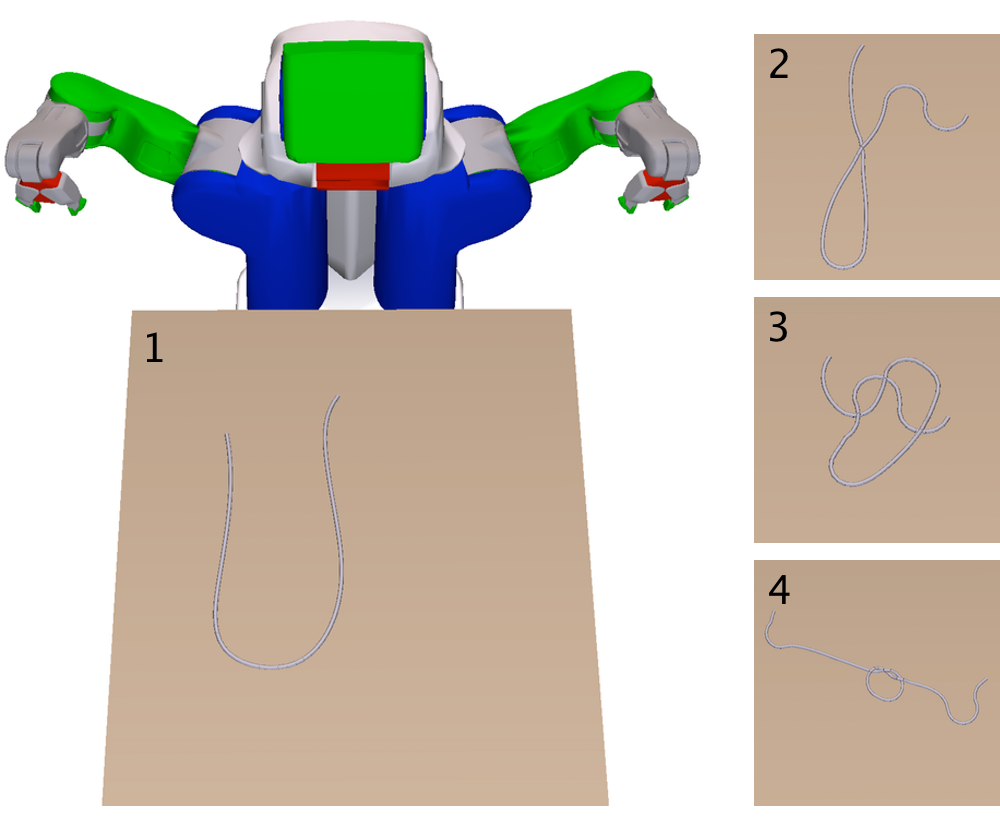
\includegraphics[width=0.45\textwidth]{figures/knot_steps_num.png}
  \caption{The overhand knot manipulation task in our benchmark.
           A standard knot tie takes three steps, as shown in this
           particular execution from our benchmark.}
  \label{fig:knot_steps}
\end{figure}

In this work, we present a solution to the demonstration selection
problem that can account for the variability in robustness of
demonstrations and incorporates the sequential nature of our
tasks. Our contributions are as follows: (i) We formulate the
demonstration selection problem as a Markov Decision Process (MDP);
(ii) We present Max-Margin Q-Learning (\mmql{}), a method for
approximating Q-functions from expert-guided task executions, based on
the optimality of the expert's action selection; (iii) We describe
task-independent features that are rich enough to allow learning but
make no additional assumptions beyond those of trajectory transfer;
and (iv) We validate this approach in a simulated knot-tying
experiment and show strong improvement over previous approaches. 

A central component of our approach is framing the demonstration
selection problem as an MDP. Given a state and a demonstration,
trajectory transfer produces an trajectory that can be executed on a
robot. Thus, given a manipulation problem and a demonstration library,
we can view the library as discretizing the action space. The savings
in this reduction can be large. For a two-armed manipulation problem
with 7DOF per arm, the action space is a parametrized trajectory with
40 intermediate poses, which is roughly $\mathbb{R}^{240}$. Using a
demonstration library will reduce the action space to a finite
set. The hope is that this discretization will still allow reasonable
solutions for the task of interest.

Using this formalism, we apply Q-learning to find a good approximate
policy to which demonstration to transfer. We introduce \mmql{} as a
method to do this with human input. The procedure combines
maximum-margin structured prediction with approximate linear
programming to learn a $Q$-function that 1) matches the human
demonstrator's $Q$-function and 2) is consistent with the dynamic
programming equations for the MDP. We improve on this approach with a
lookahead policy, which acts to maximizes the predicted $Q$-value over
a search horizon.

We developed a knot-tying benchmark for evaluating the effectiveness of
our proposed approach.   This benchmark is available at
\href{https://sites.google.com/site/rss2014mmql}{sites.google.com/site/rss2014mmql}). The
nearest neighbor approach described in \citet{Schulmanetal_ISRR2013} achieves a
68.8\% success rate on this benchmark.  The greedy policy with respect to our learned
approximate Q-function achieves a success rate of 85.6\%. Augmenting our
policy with a simulator and beam search raises the success rate to 95.2\%.

While our running example and experiments deal with knot tying, our presented
\mmql{} approach makes no assumptions about the
specifics of the task except for the availability of point clouds of
the scene.


\maketitle

%% Use plainnat to work nicely with natbib. 

\bibliographystyle{plainnat}
\bibliography{references}

\end{document}
